\documentclass[12pt]{article}
\frenchspacing
\usepackage[utf8x]{inputenc}
\usepackage[T2A]{fontenc}
\usepackage{amsmath}
\usepackage{amsfonts}
\usepackage{amssymb}
\usepackage[russian]{babel}
\usepackage{graphicx}
\usepackage{hyperref}
\usepackage{multirow}
\usepackage[left=2cm,right=2cm,top=2cm,bottom=2cm,bindingoffset=0cm]{geometry}
\author{Рашковецкий М.М., группа 526т}
\date{\today}
\title{Лабораторная работа 2.1.6\\Эффект Джоуля --- Томсона}
\begin{document}
	\maketitle
	
	{\parindent=1cm \hangindent=1cm \parskip=0.5cm
	{\bfseries Цель работы:} определение изменения температуры углекислого газа при протекании через малопроницаемую перегородку при различных начальных значенях давления и температуры; вычисление по результатам опытов коэффициентов Ван-дер-Ваальса.
	
	\hangindent=1cm
	{\bfseries Оборудование и материалы:} трубка с пористой перегородкой, труба Донера, термостат, термометр, дифференциальная термопара, микровольтметр, балластный баллон, манометр.\par}
	\section*{Краткая теория}
	
	\indent Эффект Джоуля --- Томсона --- изменение температуры газа, медленно протекающего из области высокого в область низкого давления в условиях хорошей тепловой изоляции.
	
	В работе газ переходит через пористую перегородку из области с давлением $P_1$ в область с атмосферным давлением $P_2$. Рассмотрим стационарный поток между сечениями I и II до и после перегородки. Считая стенки адиабатическими и жёсткими, из закона сохранения энергии получим:
	
	\begin{equation}
	\label{eq:energy_saving}
	A_1-A_2=\left( U_2+\frac{\nu \mu v_2^2}{2} \right) - \left( U_1+\frac{\nu \mu v_1^2}{2} \right),
	\end{equation}
	
	где $A_1=P_1 V_1$ --- работа, совершённая над газом при прохождении через I, $A_2=P_2 V_2$ --- работа, совершённая газом при прохождении через II. Тогда
	
	\begin{equation}
	\label{eq:entalpy_change}
	H_1-H_2=\frac{1}{2} \nu \mu \left( v^2_2 - v^2_1 \right).
	\end{equation}
	
	В начале опыта трение в перегородке существенно её нагревает, из-за чего \eqref{eq:energy_saving} выполняется плохо, но со временем её температура устанавливается и \eqref{eq:energy_saving} становится верным с хорошей точностью.
	
	Чистый процесс Джоуля --- Томсона (дифференциальный эффект для разреженного газа) --- когда скорости по обе стороны от перегородки малы, тогда, согласно \eqref{eq:entalpy_change}, энтальпию можем считать неизменной. Тогда
	
	\begin{equation}
	\label{eq:J-T_coeff_general}
	\mu_\text{Д---Т}=\frac{\Delta T}{\Delta P}=-\frac{\left( \partial H/ \partial P\right)_T}{\left( \partial H/ \partial T\right)_P}.
	\end{equation}
	
	Чтобы вычислить эти производные, запишем первое начало термодинамики:
	\begin{equation}
	\label{eq:first_td_law}
	\delta Q = dH-VdP.
	\end{equation}
	
	Считая $H = H \left( T,P \right)$, получим
	
	\begin{equation}
	\label{eq:first_td_law_pr}
	\delta Q = \left( \frac{\partial H}{\partial T} \right)_P dT + \left[ \left( \frac{\partial H}{\partial P} \right)_T - V \right] dP
	\end{equation}
	
	Полагая $dP=0$, по определению $C_P$ получаем
	\begin{equation}
	\label{eq:part_entalpy_temp}
	\left( \frac{\partial H}{\partial P}\right)_T = C_P.
	\end{equation}
	
	Разделим \eqref{eq:first_td_law_pr} на $T$, считая процесс квазистатическим, получаем
	\begin{equation}
	\label{eq:enthropy_diff}
	dS = \frac{1}{T} \left( \frac{\partial H}{\partial T} \right)_P dT + \frac{1}{T} \left[ \left( \frac{\partial H}{\partial P} \right)_T - V \right] dP
	\end{equation}
	
	Поскольку по второму началу термодинамики $dS$ является полным дифференциалом,
	\begin{equation}
	\label{eq:enthropy_sec_partials}
	\frac{\partial}{\partial P} \left[ \frac{1}{T} \left( \frac{\partial H}{\partial T} \right)_P \right] = \frac{\partial}{\partial T} \left\{ \frac{1}{T} \left[ \left( \frac{\partial H}{\partial P} \right)_T - V \right] \right\}
	\end{equation}
	
	После упрощения получим
	\begin{equation}
	\label{eq:part_entalpy_press}
	\left( \frac{\partial H}{\partial T}\right)_P = V-T \left( \frac{\partial V}{\partial T}\right)_P.
	\end{equation}
	
	Подставим \eqref{eq:part_entalpy_temp} и \eqref{eq:part_entalpy_press} в \eqref{eq:J-T_coeff_general}:
	\begin{equation}
	\label{eq:J-T_coeff_general_final}
	\mu_\text{Д---Т}= \left( \frac{\partial T}{\partial P}\right)_H = \frac{ T\left( \partial V/ \partial T\right)_P -V}{C_P}.
	\end{equation}
	
	Для идеального газа $PV=\nu RT$ и коэффициент Джоуля --- Томсона нулевой.
	
	Найдём коэффициент для газа Ван-дер-Ваальса. Уравнение состояния:
	\begin{equation}
	\label{eq:van-der-vaals}
	\left( P+\frac{a \nu^2}{V^2} \right) \left( \frac{V}{\nu}-b \right) = RT.
	\end{equation}
	
	Продифференцируем обе части для 1 моля газа:
	\begin{equation}
	\label{eq:van-der-vaals_diff}
	\left( dP-\frac{2a dV}{V^3} \right) \left( V-b \right) + \left( P+\frac{a}{V^2} \right) dV = RdT.
	\end{equation}
	
	Преобразуя, получим
	\begin{equation}
	\label{eq:van-der-vaals_diff2}
	\left( P-\frac{a}{V^2} + \frac{2ab}{V^3} \right) dV = RdT-\left( V-b \right) dP,
	\end{equation}
	откуда
	\begin{equation}
	\label{eq:part_vol_temp}
	\left( \frac{\partial V}{\partial T}\right)_P = \frac{R}{P-\frac{a}{V^2} + \frac{2ab}{V^3}}.
	\end{equation}
	
	Разложим по Тейлору до первого порядка:
	\begin{equation}
	\label{eq:part_vol_temp_approx}
	\left( \frac{\partial V}{\partial T}\right)_P \approx \frac{R}{P} \left( 1 +\frac{a}{PV^2} \right).
	\end{equation}
	
	Из \eqref{eq:van-der-vaals}
	\begin{equation}
	\label{eq:R_div_P}
	\frac{R}{P} = \frac{V}{T} \left( 1+\frac{a}{PV^2} \right) \left( 1-\frac{b}{V} \right).
	\end{equation}
	
	Подставим \eqref{eq:R_div_P} и \eqref{eq:part_vol_temp_approx} в \eqref{eq:J-T_coeff_general_final}, пренебрегая членами выше первого порядка (например, по \eqref{eq:van-der-vaals} $PV\approx RT$) и получим
	\begin{equation}
	\label{eq:J-T_coeff_van-der-vaals}
	\mu_\text{Д---Т} = \frac{ \frac{2a}{RT}-b}{C_P}.
	\end{equation}
	
	Отсюда видно, что для больших $a$ при расширении газ охлаждается, для малых --- нагревается. Температура, для которой эффект отсутствует и в которой меняет знак, называют температурой инверсии:
	\begin{equation}
	\label{eq:T_inv}
	T_\text{инв}=\frac{2a}{Rb}.
	\end{equation}
	
	Она связана с критической температурой как
	\begin{equation}
	\label{eq:T_inv&cr}
	T_\text{инв}=\frac{27}{4}T_\text{кр}.
	\end{equation}
	
	В таблице \ref{tbl:tinv&tcr} приведены значения критической температуры и температуры инверсии для разных газов. Из неё видно, что предсказания теории Ван-дер-Ваальса для реальных газов выполняются не очень хорошо. Она правильно передаёт их свойства качественно, но не претендует на хорошее количественное описание картины.
	
	При больших разностях давлений необходимо прибегать к более точным разложениям, приведенная теория для этого случая не годится.
	
	\begin{table}
	\caption{Критические температуры и температуры инверсии для разных газов}
	\label{tbl:tinv&tcr}
	\begin{center}
	\begin{tabular}{|c|c|c|}
	\hline
	Газ & $T_\text{кр}$, К & $T_\text{инв}$, К \\
	\hline
	Гелий & 5,2 & 46 \\
	Водород & 33 & 205 \\
	Азот & 126 & 604 \\
	Воздух & 132,6 & 650 \\
	Углекислый газ & 304 & 2050 \\
	\hline
	\end{tabular}
	\end{center}
	\end{table}
	
	Вернёмся к правой части \eqref{eq:entalpy_change}, оценим изменение температуры в связи с изменением скорости. Для этого не нужно пользоваться теорией Ван-дер-Ваальса, достаточно соотношений для идеального газа. Тогда \eqref{eq:entalpy_change} в расчёте на 1 моль преобразуется к виду
	\begin{equation}
	\label{eq:dT_vel}
	\left( C_V + R \right) \Delta T \approx \frac{\mu}{2} \left( v_2^2-v_1^2 \right)
	\end{equation}
	или
	\begin{equation}
	\label{eq:dT_vel_final}
	\Delta T \approx \frac{\mu}{2C_P} \left( v_2^2-v_1^2 \right).
	\end{equation}
	
	В опыте $Q \leqslant 10 \,\text{см}^3/ \text{с}$, $d=3\,\text{мм}$. Тогда
	\begin{equation}
	\label{eq:vel2_approx}
	v_2 \leqslant \frac{4Q}{\pi d^2} \approx 1{,}4 \text{м}/\text{с}.
	\end{equation}
	
	Для углекислого газа $\mu=44\,\text{г}/\text{моль}$, $C_P=41\,\text{Дж}/ \left( \text{моль} \cdot \text{К} \right)$, имеем
	\begin{equation}
	\label{eq:dT_vel_num}
	\Delta T \leqslant \frac{\mu}{2C_P} v_2 \approx 10^{-3} \text{K}.
	\end{equation}
	
	В работе изменение температуры порядка 1 К, так что вкладом скорости действительно можно пренебречь.
	
	\section*{Установка}
	
	\begin{figure}[h!]
	\caption{Схема установки}
	\label{fig:scheme}
	\begin{center}
	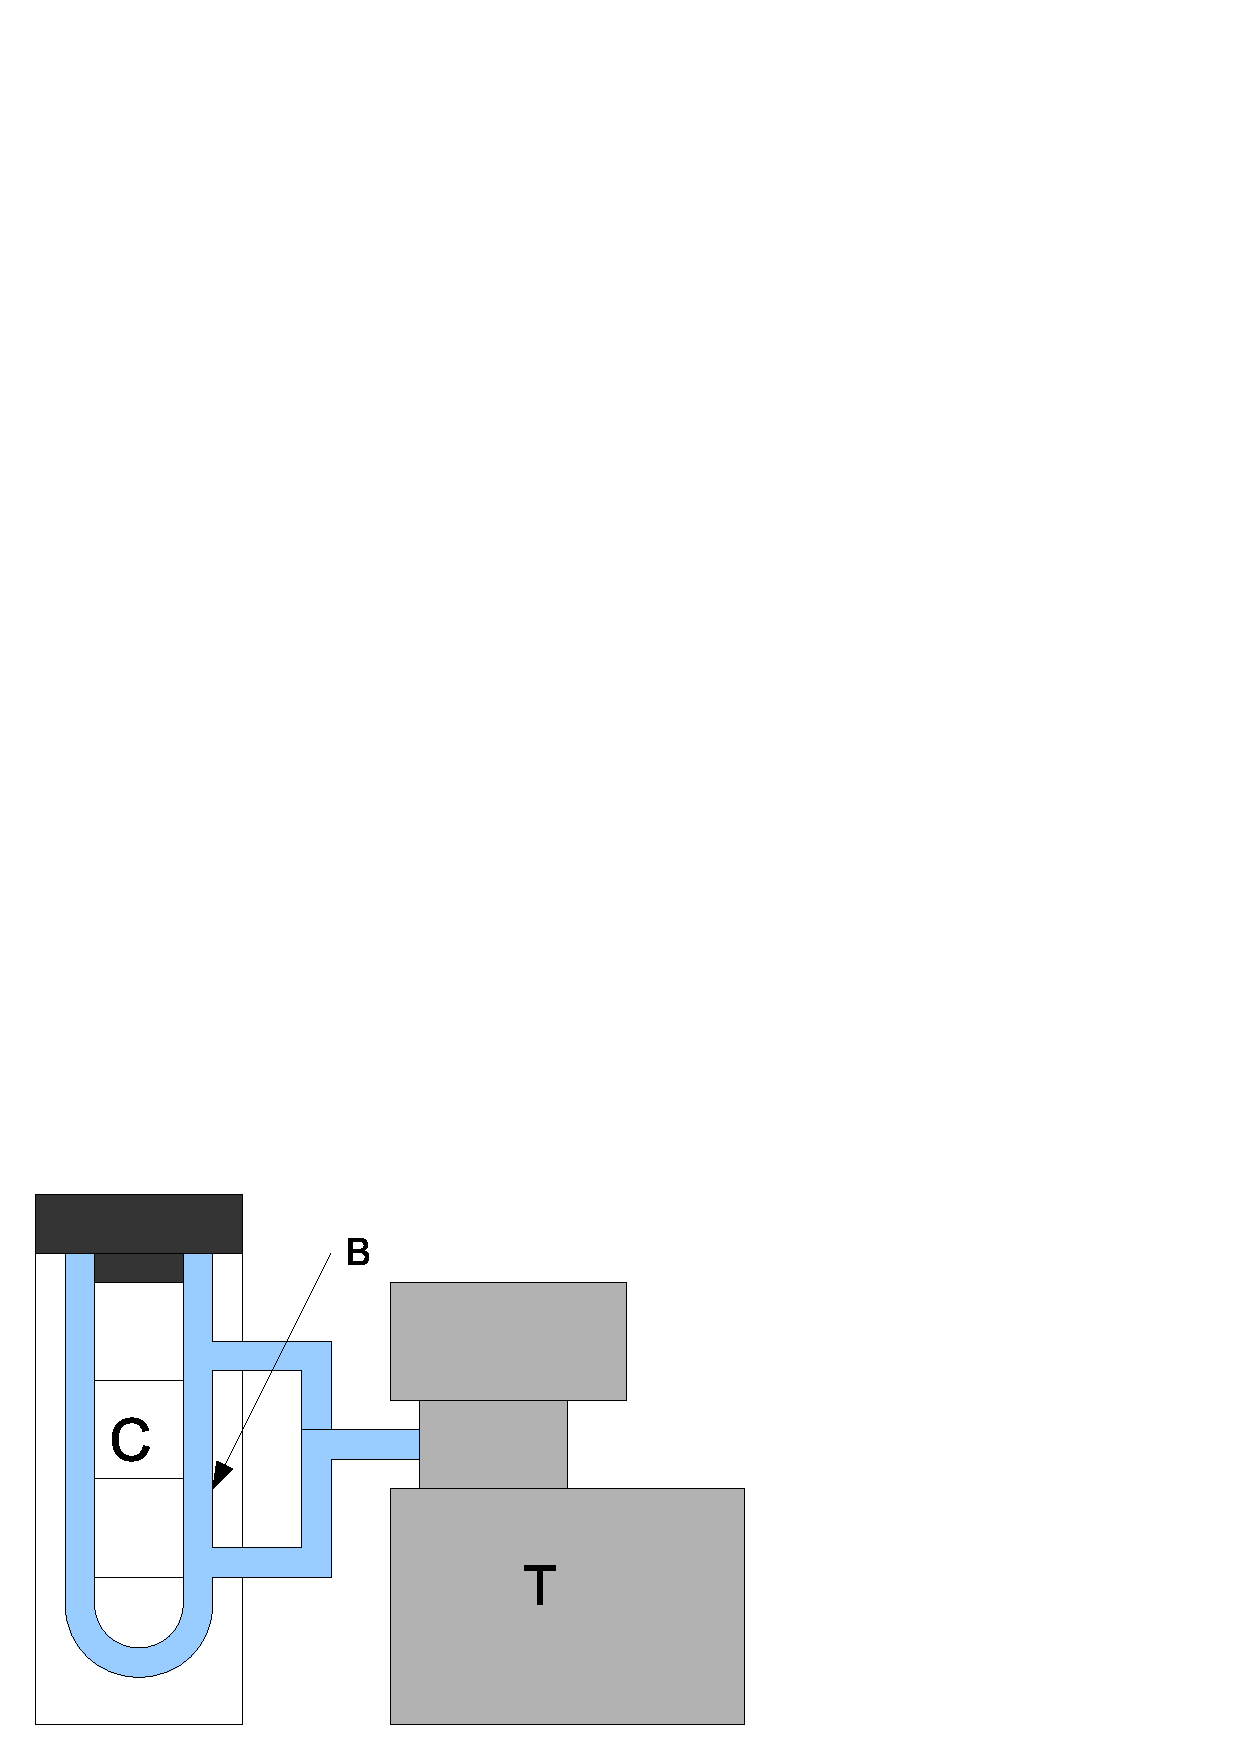
\includegraphics[scale=0.7]{scheme.png}
	\end{center}
	\end{figure}
	
	На рис. \ref{fig:scheme} приведена схема установки. Она состоит из:
	\begin{enumerate}
	\item трубки из нержавеющей стали;
	\item пористой перегородки (стеклянной пробки);
	\item теплоизолирующей трубы Дьюара, покрытой серебром для уменьшения излучения;
	\item уплотняющего кольца;
	\item змеевика, по которому поступает газ;
	\item балластного баллона;
	\item цифрового вольтметра;
	\item спая термопары после перегородки;
	\item спая термопары перед перегородкой;
	\item пробки из пенопласта.
	
	Также на схеме отмечены:
	\item кнопка включения вольтметра;
	\item кнопка <<АВП>> (автоматический выбор предела);
	\item кнопка <<U=>> (постоянный ток).
	\end{enumerate}
	
	\section*{Ход работы}
	
	\begin{enumerate}
	\item Установили на термостате температуру $t=20 ^\circ\text{C}$.
	\item Включили вольтметр на режим постоянного тока и автоматического выбора предела, записали показание $U_0$.
	\item Открыли регулирующий вентиль до предела, избыточное давление составило около 4 атм. \label{exp_loop_begin}
	\item Через 10 минут записали показания манометра и вольтметра.
	\item Снизили давление, через 5 минут записали показания манометра и вольтметра.
	\item Измерили ещё 5 точек. \label{exp_loop_end}
	\item Установили на термостате температуру $t=40 ^\circ\text{C}$. \label{exp_loop2_begin}
	\item Подождав, пока температура установится, повторили пп. \ref{exp_loop_begin}--\ref{exp_loop_end}. \label{exp_loop2_end}
	\item Повторили пп. \ref{exp_loop2_begin}--\ref{exp_loop2_end} для $t=60 ^\circ\text{C}$.
	\end{enumerate}
	
	\section*{Обработка результатов}
	
	В таблице \ref{tbl:exp_res} приведены измеренные величины: $t$, $U$ и $\Delta P$, при этом из $U$ вычтено значение при нулевой разности давлений. Чувствительность $s=U/\Delta T$ для каждой температуры взята из таблицы в лабнике, с её помощью вычислена разность температур\footnote{Здесь и далее $\Delta P$ и $\Delta T$ являются не изменениями температуры и давления при прохождении через перегородку, а убылями.}.
	
	\begin{table}[!h]
	\caption{Результаты эксперимента}
	\label{tbl:exp_res}
	\begin{center}
	\begin{tabular}{|c|c|c|c|c|}
	\hline
	$t, ^\circ\text{C}$ & $U$, мкВ & $s$, мкВ/K & $\Delta P$, атм & $\Delta T, K$ \\
	\hline
	\multirow{7}{*}{20} & 155 & \multirow{7}{*}{40,7} & 4,17 & 3,968 \\
	 & 130 &  & 3,57 & 3,353 \\
	 & 114 &  & 3,18 & 2,96 \\
	 & 99 &  & 2,88 & 2,592 \\
	 & 74 &  & 2,37 & 1,977 \\
	 & 49 &  & 1,62 & 1,363 \\
	 & 26 &  & 0,99 & 0,798 \\
	\hline
	\multirow{7}{*}{40} & 142 & \multirow{7}{*}{42,5} & 4,17 & 3,494 \\
	 & 115 &  & 3,66 & 2,858 \\
	 & 99 &  & 3,27 & 2,482 \\
	 & 69 &  & 2,46 & 1,776 \\
	 & 45 &  & 1,86 & 1,211 \\
	 & 26 &  & 1,32 & 0,764 \\
	 & 11 &  & 0,84 & 0,411 \\
	\hline
	\multirow{7}{*}{60} & 16 & \multirow{7}{*}{44,1} & 1,08 & 0,51 \\
	 & 34 &  & 1,77 & 0,918 \\
	 & 55 &  & 2,4 & 1,394 \\
	 & 75 &  & 3,03 & 1,848 \\
	 & 90 &  & 3,45 & 2,188 \\
	 & 106 &  & 3,9 & 2,551 \\
	 & 114 &  & 4.14 & 2.732 \\
	\hline
	\end{tabular}
	\end{center}
	\end{table}
	
	Затем я построил графики $\Delta T \left( \Delta P \right)$ для каждой температуры с помощью библиотеки \textbf{matplotlib} и линейно аппроксимировал их с помощью библиотеки \textbf{scipy.optimize}. Экспериментальные точки и аппроксимация нанесены на трёх графиках на рис. \ref{fig:graphs}.
	
	\begin{figure}[!h]
	\caption{Графики}
	\label{fig:graphs}
	\begin{center}
	\includegraphics[scale=0.725]{graph0.pdf}
	\includegraphics[scale=0.725]{graph1.pdf}
	\includegraphics[scale=0.725]{graph2.pdf}
	\end{center}
	\end{figure}
	
	Для каждой температуры посчитан угловой коэффициент прямой, который и является коэффициентом Джоуля --- Томсона, и его погрешность.
	
	По двум парам соседних температур посчитаны коэффициенты $a$ и $b$ в соответствии с \eqref{eq:J-T_coeff_van-der-vaals}:
	\begin{equation}
	\label{coeff_a_from_exp}
	a = \frac{R C_P}{2} \frac{\mu_1 - \mu_2}{\frac{1}{T_1}-\frac{1}{T_2}}
	\end{equation}
	\begin{equation}
	\label{coeff_b_from_exp}
	b = C_P \frac{\mu_1 T_1 - \mu_2 T_2}{T_2 - T_1}
	\end{equation}
	
	Их погрешности соответственно равны
	\begin{equation}
	\label{coeff_a_sigma}
	\sigma_a = \frac{R C_P}{2} \frac{\sqrt{\sigma^2_{\mu_1} + \sigma^2_{\mu_2}}}{\frac{1}{T_1}-\frac{1}{T_2}}
	\end{equation}
	\begin{equation}
	\label{coeff_b_sigma}
	\sigma_b = C_P \frac{\sqrt{\sigma^2_{\mu_1} T_1^2 + \sigma^2_{\mu_2} T_2^2}}{T_2 - T_1}
	\end{equation}
	
	По \eqref{eq:T_inv} посчитана температура инверсии, и оценена её погрешность как
	\begin{equation}
	\label{eq:T_inv_sigma}
	\sigma_{T_\text{инв}}=T_\text{инв} \sqrt{\left( \frac{\sigma_a}{a} \right)^2 + \left( \frac{\sigma_b}{b} \right)^2}
	\end{equation}
	
	Эти результаты, а также табличные значения $\mu_\text{Д---Т}$ при тех же температура, значения параметров $a$, $b$ при критической температуре и реальная температура инверсии приведены в таблице \ref{tbl:proc_res}.
	
	\begin{table}
	\caption{Результаты обработки и табличные данные}
	\label{tbl:proc_res}
	\begin{center}
	\begin{tabular}{|c|c|c|c|c|c|}
	\hline
	$t, ^\circ\text{C}$ & $\mu_\text{Д---Т}$, K/атм & $\mu_\text{Д---Т табл}$, K/атм & $a, \frac{\text{Н}\cdot \text{м}^4}{\text{моль}^2}$ & $b, \frac{\text{см}^3}{\text{моль}}$ & $T_\text{инв}$, K \\
	\hline
	20 & $1{,}00\pm 0{,}03$ & 1,105 & \multirow{2}{*}{$0{,}7\pm 0{,}3$} & \multirow{2}{*}{$200\pm 200$} & \multirow{2}{*}{$900\pm 1500$} \\
	\multirow{2}{*}{40} & \multirow{2}{*}{$0{,}91\pm 0{,}03$} & \multirow{2}{*}{0,958} & & & \\
		&	&	&	\multirow{2}{*}{$1{,}6\pm 0{,}3$} & \multirow{2}{*}{$800\pm 200$} & \multirow{2}{*}{$450\pm 40$} \\
	60 & $0{,}737\pm 0{,}015$ & 0,838 & & & \\
	\hline
	31 & --- & --- & 0,3652 & 42,792 & 2053 \\
	\hline
	\end{tabular}
	\end{center}
	\end{table}
	
	Значения коэффициентов Джоуля --- Томсона отклоняются от табличных приблизтельно на 10\%, однако более чем на $3 \sigma$. Это может быть связано с тем, что мы недостаточно долго ждали установления показаний вольтметра, с наличием примесей или тем, что погрешности занижены.
	
	Средние значения параметров из уравнения Ван-дер-Ваальса, полученные по паре температур $20 ^\circ\text{C}$ и $40 ^\circ\text{C}$, ближе к табличным, как и ожидалось, поскольку температуры ближе к критической. Однако для коэффициента $b$ и температуры инверсии в этом случае погрешности превысили 100\%, это говорит о том, что точности эксперимента не хватает, чтобы уловить их значения. Для пары $40 ^\circ\text{C}$ и $60 ^\circ\text{C}$ параметры отличаются от табличных уже очень сильно, из чего можно сделать вывод, что реальный газ достаточно далёк от модели Ван-дер-Ваальса.
	
\end{document}
